% Második előadás

\chapter{Nagy teljesítményű, két foglalatos szerver processzorok fejlődése}

\section{Szerver platformok osztályozása}
A szerver rendszerek feloszthatók egy processzoros (UP) és több processzoros platformokra.
A több processzoros platformok feloszthatók két foglalatos (2S/DP), négy vagy nyolc foglalatos (4S, 8S) és nyolcnál több foglalatos rendszerekre.
A piac nagy részét a két processzoros szerverek teszik ki (kb. 80\%), ezért részletesebben ezekkel foglalkozunk.

\section{Méret, tranzisztorok}
A 2S szerver processzorok nagy méretűek, sok tranzisztort tartalmaznak.
A 2000-es évek közepén a Pentium 4 szerver processzorok még viszonylag kevés tranzisztorból álltak (125 millió), ezért elég volt kb 1 cm\textsuperscript{2}-es lapka.
A magok számának növekedésével egyre több tranzisztor kellett, a Skylake (2017) processzoroknál már 8 milliárd.
Még újabb CPU-knál nincs információ.
Ezzel együtt a lapkaméret is tovább nőtt, a mai lapkáknál 8 cm\textsuperscript{2} körüli.

Mivel a lapkák gyártása nagyon komplex, nagyobb méretű lapkáknál több hiba előfordulhat, ezért alacsonyabb lesz a kihozatali arány.
A lapkák méretét így a gazdasági hatékonyság is meghatározza.

\section{Fogyasztás}
A HEDT processzoroknál is nagyobb fogyasztással kell számolni a szerver processzoroknál, 130-tól 200 W felettig mennek.

\section{Lábak száma}
A szerver processzorok sok lábbal kapcsolódnak a foglalatokhoz, amik precíz gyártást igényelnek.

\section{Magok száma}
A szerver alkalmazások általában jól párhuzamosíthatók, így a processzorok a lehető legtöbb magot implementálják.
A Pentium 4 szerver processzoránál még csak 1 mag volt, de később 28-ig növekedett a magok száma.

\section{Intel Cascade Lake 9200-AP}
Ez a 2x28, azaz 56 magos processzor az Intel válasza volt az AMD 64 magos EPYC Rome processzoraira.
Az AMD 2017-ben adta ki ezt a processzort, ami valós konkurenciát állított az Intelnek, ami 2015 környékén még nagyrészt egyeduralkodó volt a szervereknél.
Ezért az Intel két 28 magos lapkát tett egy foglalatba, és BGA (Ball Grid Array) tokozással látta el, ami forrasztásra készült.
A forrasztás miatt nem voltak külön megvásárolhatók, csak OEM-ek kapták meg.

A két lapka egybecsomagolása miatt egy két foglalatos rendszer gyakorlatilag 4 processzort jelent.

\section{Magszámok és tranzisztorok növekedése}
A kétfoglalatos szerver CPU-k esetében kb 2 évente duplázódott a magok száma (\ref{fig:core}. ábra).

\begin{figure}[H]
    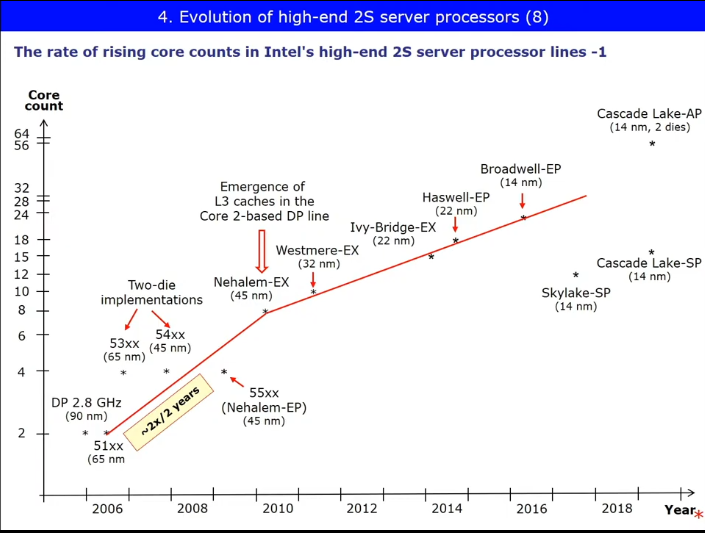
\includegraphics[width=0.8\textwidth]{core}
    \centering
    \caption{Intel 2S szerver processzorok magszámának fejlődése}
    \label{fig:core}
\end{figure}

Ez összhangban van a Moore-szabállyal, ami szerint a tranzisztorok száma két évente duplázódik.
Az utóbbi években viszont lelassult a fejlődés, már csak négy évente duplázódott a magok száma.
Ennek egyik oka az L3 cache megjelenése, ami elfoglalja a lapka jelentős részét, mivel nagyon sok tranzisztor kell a működéséhez.
A technológi változása miatt a Moore törvénnyel ellentétben az Intel már csak 4 évente tudta duplázni a tranzisztorok számát (\ref{fig:transistor}. ábra).
Ennek az oka, hogy a sok tranzisztor disszipációját kezelni kell, ami korlátozza a fejlődést.

\begin{figure}[H]
    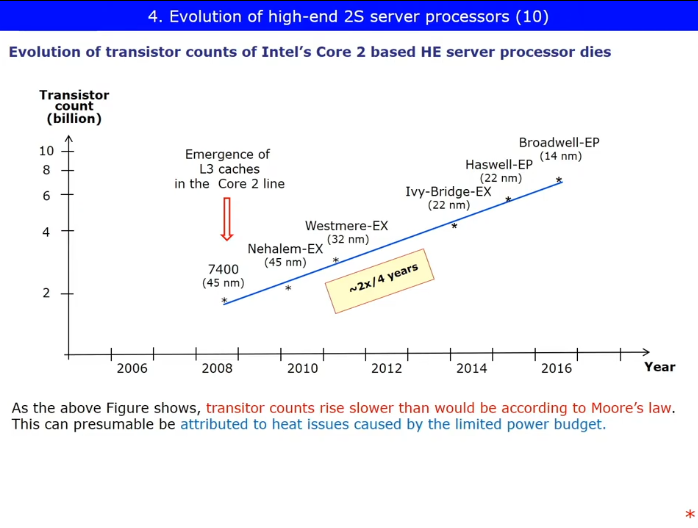
\includegraphics[width=0.8\textwidth]{transistor}
    \centering
    \caption{Intel 2S szerver processzorok tranzisztorszámának fejlődése}
    \label{fig:transistor}
\end{figure}

\subsection{Kivételek}
Néhány processzor az ábrán nem illik a fejlődési görbére, ezek az AMD konkurenciára adott válaszoknak köszönhetők.

\section{Memória sebességek fejlődése}
A memória sebességeknél adatátviteli rátával jellemezzük őket, mivel a frekvencia nem azonos az átviteli sebességgel a DDR (Double Data Rate) memóriák esetében.

\begin{figure}[H]
    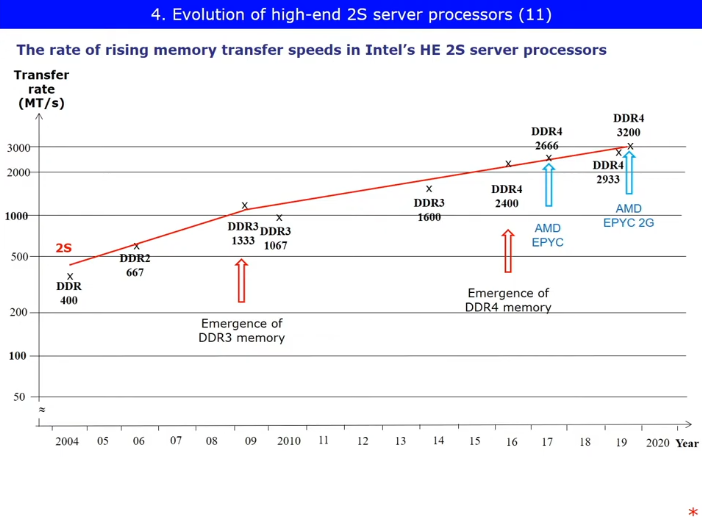
\includegraphics[width=0.8\textwidth]{mem}
    \centering
    \caption{Memória sebességek fejlődése}
    \label{fig:mem}
\end{figure}

A \ref{mem}. ábrán látható, hogy a DDR és DDR2-es memóriák gyorsabban fejlődtek, mint a DDR3 és DDR4 memóriák.
Az első szakaszban egy duplázódáshoz 4 év kellett, DDR3 óta pedig már 8.
Ennek oka a DDR3-as memóriák jóval komplexebb felépítése, ami lassította a fejlődést.
A magok száma tehát gyorsabban növekedett, mint a memóriák sebessége, ami konfliktusforrás.

Szerverek esetében elvárás, hogy az egymástól függetlenül működő magokat azonos memória sávszélességgel kell ellátni.
Tehát a sávszélességet lineárisan skálázni kell a magszámmal együtt.
A foglalatonkénti sávszélesség kiszámítása:
\begin{equation}
    BW/core = n_M*w*T_M/n_C
\end{equation}
ahol:
\begin{itemize}
    \item n\textsubscript{M}: memória csatornák száma
    \item w: memória csatorna szélessége (pl. 8 byte)
    \item T\textsubscript{M}: memória átviteli rátája (pl. 2.4 GT/s)
    \item n\textsubscript{C}: magok száma
\end{itemize}

Probléma, hogy a transzfer ráta lassabban nő, mint a magok száma, tehát $T_m/n_C$ folyamatosan csökken.
Megoldás a memória csatornák számának növelése.
Ez azonban elég komplex feladat.

A magonkénti memória sávszélességnél referenciának tekinthető a Pentium 4 DP rendszer, a fejlesztési cél ehhez az értékhez tartani.
